%%%%%%%%%%%%%%%%%%%%%%%%%%%%%%%%%%%%%%%%%%%%%%%%%%%%%%%%%%%%%%%%%
%%  To create image run: (for Windows use imgconvert)
%%
%%  convert -verbose -delay 50 -loop 0 -density 300 -resize 640x480 <name>.pdf <name>.gif
%%
%%%%%%%%%%%%%%%%%%%%%%%%%%%%%%%%%%%%%%%%%%%%%%%%%%%%%%%%%%%%%%%%
\documentclass[beamer,tikz,preview]{standalone}
%\documentclass{beamer}

\setbeamertemplate{navigation symbols}{}
\usepackage{tikz}
\usepackage{color}

\tikzset{pics/.cd,
cube/.style args={#1/#2/#3/#4}{code={
\coordinate (O) at (0,0,0);
\coordinate (A) at (0,#2,0);
\coordinate (B) at (0,#2,#3);
\coordinate (C) at (0,0,#3);
\coordinate (D) at (#1,0,0);
\coordinate (E) at (#1,#2,0);
\coordinate (F) at (#1,#2,#3);
\coordinate (G) at (#1,0,#3);
\draw[black,fill=black!80] (O) -- (C) -- (G) -- (D) -- cycle;
\draw[black,fill=black!30] (O) -- (A) -- (E) -- (D) -- cycle;
\draw[black,fill=black!10] (O) -- (A) -- (B) -- (C) -- cycle;
\draw[black,fill=black!20,opacity=0.8] (D) -- (E) -- (F) -- (G) -- cycle;
\draw[black,fill=black!20,opacity=0.6] (C) -- (B) -- (F) -- (G) -- cycle;
\draw[black,fill=black!20,opacity=0.8] (A) -- (B) -- (F) -- (E) -- cycle;
\node at (0.5*#1,0.5*#2,0.5*#3) {#4};
}}}
\tikzset{pics/.cd,
lwing/.style args={#1/#2/#3/#4}{code={
\coordinate (O) at ( 0, 0, 0);
\coordinate (A) at ( 0, 0,#3);
\coordinate (B) at ( 0,#2,#3);
\coordinate (C) at ( 0,#2, 0);
\draw[black,fill=red!20] (O) -- (A) -- (B) -- (C) -- cycle;
\node at (0,0.5*#2,0.5*#3) {#4};
}}}
\tikzset{pics/.cd,
mwing/.style args={#1/#2/#3/#4}{code={
\coordinate (O) at ( 0, 0, 0);
\coordinate (A) at (#1, 0, 0);
\coordinate (B) at (#1,#2, 0);
\coordinate (C) at ( 0,#2, 0);
\draw[black,fill=green!20] (O) -- (A) -- (B) -- (C) -- cycle;
\node at (0.5*#1,0.5*#2,0) {#4};
}}}
\tikzset{pics/.cd,
rwing/.style args={#1/#2/#3/#4}{code={
\coordinate (O) at ( 0, 0, 0);
\coordinate (A) at (#1, 0, 0);
\coordinate (B) at (#1, 0,#3);
\coordinate (C) at ( 0, 0,#3);
\draw[black,fill=blue!20] (O) -- (A) -- (B) -- (C) -- cycle;
\node at (0.5*#1,0,0.5*#3) {#4};
}}}

\begin{document}
\begin{frame}

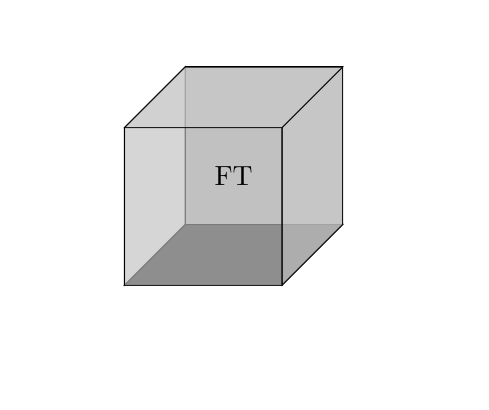
\begin{tikzpicture}
    \pic at (0,0,0) {cube={2/2/2/T}};
    \pic at (0,0,2) {lwing={2/2/2/F}};

\pause
\fill[color=white] (-2,-2,0) rectangle (3.5,2.5,0);

    \pic at (0,0,0) {cube={0.5/2/2/$T_1$}};
    \pic at (0,0,2) {lwing={2/2/2/F}};
    \pic at (2.5,0,0) {cube={0.5/2/2/$T_d$}};
    \pic at (2.5,0,2) {lwing={2/2/2/F}};
    \draw[dashed] (0,0,2) -- (1.75,0,2);
    \draw[dashed] (0,2,2) -- (3,2,2);
    \draw[dashed] (0,2,0) -- (3,2,0);

\pause
\fill[color=white] (-2,-2,0) rectangle (3.5,2.5,0);

    \pic at (0,0,0) {cube={0.5/2/2/$FT_1$}};
    \pic at (1.75,0,0) {cube={0.5/2/2/$FT_d$}};
    \draw[dashed] (0,0,2) -- (1.75,0,2);
    \draw[dashed] (0,2,2) -- (2,2,2);
    \draw[dashed] (0,2,0) -- (2,2,0);

\pause
\fill[color=white] (-2,-2,0) rectangle (3.5,2.5,0);

    \pic at (0,0,0) {cube={2/2/2/FT}};

\end{tikzpicture}

\end{frame}

\end{document}